\documentclass[a4paper]{article}

\usepackage[english]{babel}
\usepackage[utf8]{inputenc}
\usepackage{graphicx}
\usepackage[colorinlistoftodos]{todonotes}
\usepackage{listings}
\usepackage{xcolor}

\lstset{
    frame=tb,
    tabsize=4,
    showstringspaces=false,
    numbers=left,
    commentstyle=\color{green},
    keywordstyle=\color{blue},
    stringstyle=\color{red}
}

\title{Breakable Actor}

\author{Edward Seim}

\date{Novemeber 12, 2014}

\begin{document}

\maketitle

\section{Summary}

Creating an actor that breaks is one of the more unique things I've had to make in Unreal. I didn't have to program a blueprint or C++, everything needed to do make it already exists in Unreal. You take a regular mesh and simply tell the editor to create a breakable mesh. I then lets you customize how it breaks and into the number of pieces you want. You don't necessrily get to chose certain parts to be broken up into a certain way, it just picks the points to break for you.

\section{Snapshot}

\begin{figure}
\centering
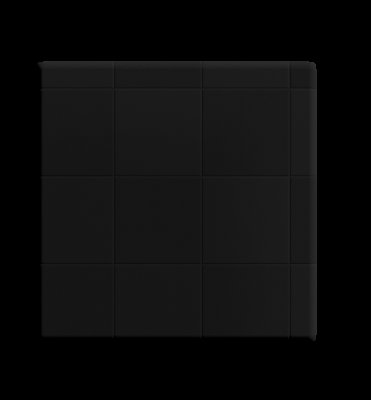
\includegraphics[keepaspectratio=true, scale=.4]{CompleteCube.png}
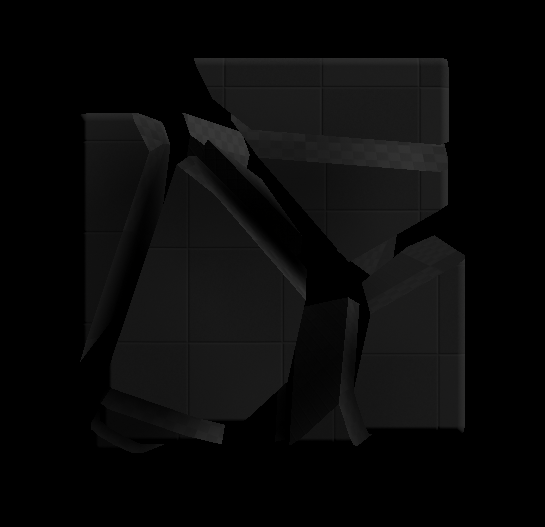
\includegraphics[keepaspectratio=true, scale=.4]{BrokenCube.png}
\end{figure}

\end{document}